\documentclass[twoside]{book}

% Packages required by doxygen
\usepackage{fixltx2e}
\usepackage{calc}
\usepackage{doxygen}
\usepackage{graphicx}
\usepackage[utf8]{inputenc}
\usepackage{makeidx}
\usepackage{multicol}
\usepackage{multirow}
\PassOptionsToPackage{warn}{textcomp}
\usepackage{textcomp}
\usepackage[nointegrals]{wasysym}
\usepackage[table]{xcolor}

% NLS support packages
\usepackage[catalan]{babel}

% Font selection
\usepackage[T1]{fontenc}
\usepackage{mathptmx}
\usepackage[scaled=.90]{helvet}
\usepackage{courier}
\usepackage{amssymb}
\usepackage{sectsty}
\renewcommand{\familydefault}{\sfdefault}
\allsectionsfont{%
  \fontseries{bc}\selectfont%
  \color{darkgray}%
}
\renewcommand{\DoxyLabelFont}{%
  \fontseries{bc}\selectfont%
  \color{darkgray}%
}
\newcommand{\+}{\discretionary{\mbox{\scriptsize$\hookleftarrow$}}{}{}}

% Page & text layout
\usepackage{geometry}
\geometry{%
  a4paper,%
  top=2.5cm,%
  bottom=2.5cm,%
  left=2.5cm,%
  right=2.5cm%
}
\tolerance=750
\hfuzz=15pt
\hbadness=750
\setlength{\emergencystretch}{15pt}
\setlength{\parindent}{0cm}
\setlength{\parskip}{0.2cm}
\makeatletter
\renewcommand{\paragraph}{%
  \@startsection{paragraph}{4}{0ex}{-1.0ex}{1.0ex}{%
    \normalfont\normalsize\bfseries\SS@parafont%
  }%
}
\renewcommand{\subparagraph}{%
  \@startsection{subparagraph}{5}{0ex}{-1.0ex}{1.0ex}{%
    \normalfont\normalsize\bfseries\SS@subparafont%
  }%
}
\makeatother

% Headers & footers
\usepackage{fancyhdr}
\pagestyle{fancyplain}
\fancyhead[LE]{\fancyplain{}{\bfseries\thepage}}
\fancyhead[CE]{\fancyplain{}{}}
\fancyhead[RE]{\fancyplain{}{\bfseries\leftmark}}
\fancyhead[LO]{\fancyplain{}{\bfseries\rightmark}}
\fancyhead[CO]{\fancyplain{}{}}
\fancyhead[RO]{\fancyplain{}{\bfseries\thepage}}
\fancyfoot[LE]{\fancyplain{}{}}
\fancyfoot[CE]{\fancyplain{}{}}
\fancyfoot[RE]{\fancyplain{}{\bfseries\scriptsize Generat a Dl Dec 14 2015 21\+:01\+:36 per a P\+A\+C3 per Doxygen }}
\fancyfoot[LO]{\fancyplain{}{\bfseries\scriptsize Generat a Dl Dec 14 2015 21\+:01\+:36 per a P\+A\+C3 per Doxygen }}
\fancyfoot[CO]{\fancyplain{}{}}
\fancyfoot[RO]{\fancyplain{}{}}
\renewcommand{\footrulewidth}{0.4pt}
\renewcommand{\chaptermark}[1]{%
  \markboth{#1}{}%
}
\renewcommand{\sectionmark}[1]{%
  \markright{\thesection\ #1}%
}

% Indices & bibliography
\usepackage{natbib}
\usepackage[titles]{tocloft}
\setcounter{tocdepth}{3}
\setcounter{secnumdepth}{5}
\makeindex

% Hyperlinks (required, but should be loaded last)
\usepackage{ifpdf}
\ifpdf
  \usepackage[pdftex,pagebackref=true]{hyperref}
\else
  \usepackage[ps2pdf,pagebackref=true]{hyperref}
\fi
\hypersetup{%
  colorlinks=true,%
  linkcolor=blue,%
  citecolor=blue,%
  unicode%
}

% Custom commands
\newcommand{\clearemptydoublepage}{%
  \newpage{\pagestyle{empty}\cleardoublepage}%
}


%===== C O N T E N T S =====

\begin{document}

% Titlepage & ToC
\hypersetup{pageanchor=false,
             bookmarks=true,
             bookmarksnumbered=true,
             pdfencoding=unicode
            }
\pagenumbering{roman}
\begin{titlepage}
\vspace*{7cm}
\begin{center}%
{\Large P\+A\+C3 \\[1ex]\large 3.\+0 }\\
\vspace*{1cm}
{\large Generat per Doxygen 1.8.7}\\
\vspace*{0.5cm}
{\small Dl Dec 14 2015 21:01:36}\\
\end{center}
\end{titlepage}
\clearemptydoublepage
\tableofcontents
\clearemptydoublepage
\pagenumbering{arabic}
\hypersetup{pageanchor=true}

%--- Begin generated contents ---
\chapter{Índex de Fitxers}
\section{Llista dels Fitxers}
Aquesta és la llista de tots els fitxers acompanyats amb breus descripcions\+:\begin{DoxyCompactList}
\item\contentsline{section}{P\+A\+C3-\/\+U\+O\+C/libsrc/\hyperlink{filtres_8c}{filtres.\+c} \\*Codi font de diferents funcions que serveixen per filtrar un text donat com a paràmetre d'entrada en format .txt }{\pageref{filtres_8c}}{}
\item\contentsline{section}{P\+A\+C3-\/\+U\+O\+C/libsrc/\hyperlink{filtres_8h}{filtres.\+h} \\*Capçaleres de les funcions de \hyperlink{filtres_8c}{filtres.\+c} }{\pageref{filtres_8h}}{}
\end{DoxyCompactList}

\chapter{Documentació dels Fitxers}
\hypertarget{filtres_8c}{\section{Referència del Fitxer P\+A\+C3-\/\+U\+O\+C/libsrc/filtres.c}
\label{filtres_8c}\index{P\+A\+C3-\/\+U\+O\+C/libsrc/filtres.\+c@{P\+A\+C3-\/\+U\+O\+C/libsrc/filtres.\+c}}
}


Codi font de diferents funcions que serveixen per filtrar un text donat com a paràmetre d'entrada en format .txt.  


{\ttfamily \#include $<$unistd.\+h$>$}\\*
{\ttfamily \#include $<$stdlib.\+h$>$}\\*
{\ttfamily \#include $<$string.\+h$>$}\\*
{\ttfamily \#include $<$stdio.\+h$>$}\\*
{\ttfamily \#include \char`\"{}filtres.\+h\char`\"{}}\\*
Inclou el graf de dependències per a filtres.\+c\+:\nopagebreak
\begin{figure}[H]
\begin{center}
\leavevmode
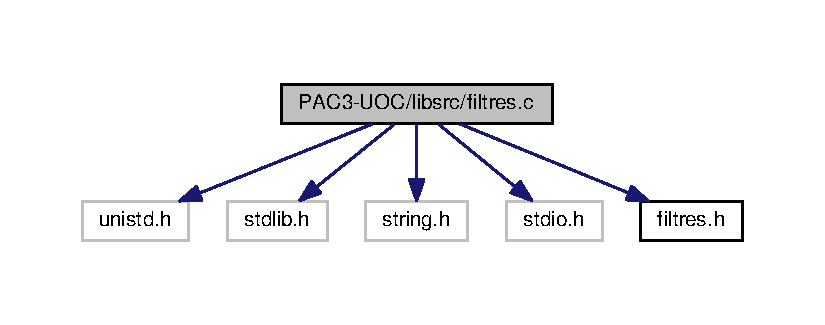
\includegraphics[width=350pt]{filtres_8c__incl}
\end{center}
\end{figure}
\subsection*{Funcions}
\begin{DoxyCompactItemize}
\item 
void \hyperlink{filtres_8c_a6bc4e3de38e285d91873339766f429b8}{printstr} (int num)
\begin{DoxyCompactList}\small\item\em Funció que imprimix per pantalla el número donat en el paràmetre d'entrada. \end{DoxyCompactList}\item 
void \hyperlink{filtres_8c_a70af81d8e422b34c60277715a0bf44f5}{fs\+\_\+head} (int fd)
\begin{DoxyCompactList}\small\item\em Funció que imprimix per pantalla les tres primeres línees. \end{DoxyCompactList}\item 
void \hyperlink{filtres_8c_afd7a1b36922bf518c9bd7e8a848df96a}{fs\+\_\+wc} (int fd)
\begin{DoxyCompactList}\small\item\em Funció que conta el nombre de caràcters, paraules i línies. \end{DoxyCompactList}\item 
void \hyperlink{filtres_8c_a643063470b5a645fd962404c2850c3bd}{fs\+\_\+nl} (int fd)
\begin{DoxyCompactList}\small\item\em Filtre que numera les línies de l'entrada i ho trau per pantalla. \end{DoxyCompactList}\item 
void \hyperlink{filtres_8c_a9a8dabec27d785f7ec81e8a498b9f5a3}{fs\+\_\+cut} (int fd, int col)
\begin{DoxyCompactList}\small\item\em Filtre que mostra la paraula a la posició col de cada línia, la primera paraula de cada línia està a la posició 1, no 0. \end{DoxyCompactList}\end{DoxyCompactItemize}


\subsection{Descripció Detallada}
Codi font de diferents funcions que serveixen per filtrar un text donat com a paràmetre d'entrada en format .txt. 

Les funcions són\+:

void \hyperlink{filtres_8c_a70af81d8e422b34c60277715a0bf44f5}{fs\+\_\+head( int fd )} Filtre que mostra les tres primeres línies de l'arxiu i ho mostra per pantalla. Les línies estan separades pel caràcter salt de línia.

void \hyperlink{filtres_8c_afd7a1b36922bf518c9bd7e8a848df96a}{fs\+\_\+wc( int fd )} Filtre que conta el nombre de caràcters, paraules i línies de l'arxiu d'entrada i ho mostra per pantalla.

void \hyperlink{filtres_8c_a643063470b5a645fd962404c2850c3bd}{fs\+\_\+nl( int fd )} Filtre que numera les línies de l'entrada i ho trau per pantalla.

void \hyperlink{filtres_8c_a9a8dabec27d785f7ec81e8a498b9f5a3}{fs\+\_\+cut( int fd, int col )} Filtre que mostra la paraula a la posició col de cada línia, la primera paraula de cada línia està a la posició 1, no 0.

\begin{DoxyAuthor}{Autor}
Alfredo Rafael Vicente Boix i Eduardo César Galobardes 
\end{DoxyAuthor}
\begin{DoxyDate}{Data}
14/12/2015 
\end{DoxyDate}


Definició al fitxer \hyperlink{filtres_8c_source}{filtres.\+c}.



\subsection{Documentació de les Funcions}
\hypertarget{filtres_8c_a9a8dabec27d785f7ec81e8a498b9f5a3}{\index{filtres.\+c@{filtres.\+c}!fs\+\_\+cut@{fs\+\_\+cut}}
\index{fs\+\_\+cut@{fs\+\_\+cut}!filtres.\+c@{filtres.\+c}}
\subsubsection[{fs\+\_\+cut}]{\setlength{\rightskip}{0pt plus 5cm}void fs\+\_\+cut (
\begin{DoxyParamCaption}
\item[{int}]{fd, }
\item[{int}]{col}
\end{DoxyParamCaption}
)}}\label{filtres_8c_a9a8dabec27d785f7ec81e8a498b9f5a3}


Filtre que mostra la paraula a la posició col de cada línia, la primera paraula de cada línia està a la posició 1, no 0. 

Aquest filtre mostra la paraula a la posició col, que és un paràmetre que s'ha de proporcionar a la funció, de cada línia. El filtre comença a contar per la paraula 1 i a continuació la segona, i així fins acabar. Si no hi ha prou columnes en la línea, la obvia i no la té en compte de manera que una línea amb 3 paraules i donant-\/li com a paràmetre d'entrada 4, no mostraria res per pantalla i passaria a la següent línea.


\begin{DoxyParams}{Paràmetres}
{\em fd} & enter que proporcionar l'identificador de l'arxiu que hem obert per a poder filtrar. \\
\hline
{\em col} & enter que indica quin és el número de columna que es vol mostrat de cada línea. \\
\hline
\end{DoxyParams}
\begin{DoxyReturn}{Retorna}
void la funció no torna cap valor 
\end{DoxyReturn}


Definició a la línia 160 del fitxer filtres.\+c.

\hypertarget{filtres_8c_a70af81d8e422b34c60277715a0bf44f5}{\index{filtres.\+c@{filtres.\+c}!fs\+\_\+head@{fs\+\_\+head}}
\index{fs\+\_\+head@{fs\+\_\+head}!filtres.\+c@{filtres.\+c}}
\subsubsection[{fs\+\_\+head}]{\setlength{\rightskip}{0pt plus 5cm}void fs\+\_\+head (
\begin{DoxyParamCaption}
\item[{int}]{fd}
\end{DoxyParamCaption}
)}}\label{filtres_8c_a70af81d8e422b34c60277715a0bf44f5}


Funció que imprimix per pantalla les tres primeres línees. 

Aquest filtre mostrarà les tres primeres línies llegides. Les línies estan separades pel caràcter salt de línia.


\begin{DoxyParams}{Paràmetres}
{\em fd} & enter que proporcionar l'identificador de l'arxiu que hem obert per a poder filtrar.\\
\hline
\end{DoxyParams}
\begin{DoxyReturn}{Retorna}
void la funció no torna cap valor 
\end{DoxyReturn}


Definició a la línia 69 del fitxer filtres.\+c.

\hypertarget{filtres_8c_a643063470b5a645fd962404c2850c3bd}{\index{filtres.\+c@{filtres.\+c}!fs\+\_\+nl@{fs\+\_\+nl}}
\index{fs\+\_\+nl@{fs\+\_\+nl}!filtres.\+c@{filtres.\+c}}
\subsubsection[{fs\+\_\+nl}]{\setlength{\rightskip}{0pt plus 5cm}void fs\+\_\+nl (
\begin{DoxyParamCaption}
\item[{int}]{fd}
\end{DoxyParamCaption}
)}}\label{filtres_8c_a643063470b5a645fd962404c2850c3bd}


Filtre que numera les línies de l'entrada i ho trau per pantalla. 

Aquest filtre numera les línies de l'entrada, de manera que queden numerades de la següent manera\+:
\begin{DoxyEnumerate}
\item Primera línea.
\item Segona línea.
\item etc...
\end{DoxyEnumerate}


\begin{DoxyParams}{Paràmetres}
{\em fd} & enter que proporcionar l'identificador de l'arxiu que hem obert per a poder filtrar.\\
\hline
\end{DoxyParams}
\begin{DoxyReturn}{Retorna}
void la funció no torna cap valor 
\end{DoxyReturn}


Definició a la línia 131 del fitxer filtres.\+c.

\hypertarget{filtres_8c_afd7a1b36922bf518c9bd7e8a848df96a}{\index{filtres.\+c@{filtres.\+c}!fs\+\_\+wc@{fs\+\_\+wc}}
\index{fs\+\_\+wc@{fs\+\_\+wc}!filtres.\+c@{filtres.\+c}}
\subsubsection[{fs\+\_\+wc}]{\setlength{\rightskip}{0pt plus 5cm}void fs\+\_\+wc (
\begin{DoxyParamCaption}
\item[{int}]{fd}
\end{DoxyParamCaption}
)}}\label{filtres_8c_afd7a1b36922bf518c9bd7e8a848df96a}


Funció que conta el nombre de caràcters, paraules i línies. 

Aquest filtre contarà el nombre de caràcters, paraules i línies de l'entrada i ho mostrarà per pantalla. Es consideren com a separadors de paraules els caràcters salt de línia, tabulador i espai en blanc; i com a separador de línies només el salt de línia. Dues paraules poden estar separades per diversos caràcters separadors.


\begin{DoxyParams}{Paràmetres}
{\em fd} & enter que proporcionar l'identificador de l'arxiu que hem obert per a poder filtrar.\\
\hline
\end{DoxyParams}
\begin{DoxyReturn}{Retorna}
void la funció no torna cap valor 
\end{DoxyReturn}


Definició a la línia 93 del fitxer filtres.\+c.

\hypertarget{filtres_8c_a6bc4e3de38e285d91873339766f429b8}{\index{filtres.\+c@{filtres.\+c}!printstr@{printstr}}
\index{printstr@{printstr}!filtres.\+c@{filtres.\+c}}
\subsubsection[{printstr}]{\setlength{\rightskip}{0pt plus 5cm}void printstr (
\begin{DoxyParamCaption}
\item[{int}]{num}
\end{DoxyParamCaption}
)}}\label{filtres_8c_a6bc4e3de38e285d91873339766f429b8}


Funció que imprimix per pantalla el número donat en el paràmetre d'entrada. 

Amb aquesta funció fem la reserva de memòria necessària per a possar en memòria els enters passats en el paràmetre d'entrada que s'alliberarà posteriorment. Després es crea una cadena de tipus \char`\"{}1. \char`\"{} que es passa per a ser escrita per pantalla. Si la funció presenta cap error es deixa d'executar i no s'allibera la memòria. Si es desitja modificar aquest punt es pot utlitzar la següent modificació\+: \begin{DoxyVerb}if(write( 1, nstr, strlen( nstr ) ) == -1){free (nstr); exit;}
\end{DoxyVerb}



\begin{DoxyParams}{Paràmetres}
{\em num} & enter proporcionat per a ser escrit per pantalla.\\
\hline
\end{DoxyParams}
\begin{DoxyReturn}{Retorna}
void la funció no torna cap valor 
\end{DoxyReturn}


Definició a la línia 40 del fitxer filtres.\+c.


\hypertarget{filtres_8h}{\section{Referència del Fitxer P\+A\+C3-\/\+U\+O\+C/libsrc/filtres.h}
\label{filtres_8h}\index{P\+A\+C3-\/\+U\+O\+C/libsrc/filtres.\+h@{P\+A\+C3-\/\+U\+O\+C/libsrc/filtres.\+h}}
}


Capçaleres de les funcions de \hyperlink{filtres_8c}{filtres.\+c}.  


Aquest gràfic mostra quins fitxers inclouen, de forma directa o indirecta, aquest fitxer\+:\nopagebreak
\begin{figure}[H]
\begin{center}
\leavevmode
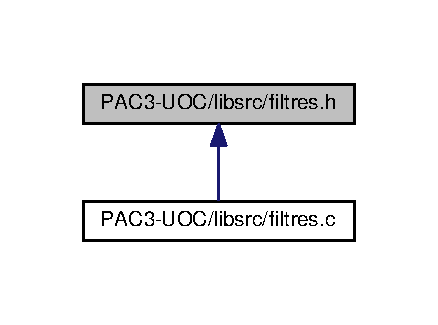
\includegraphics[width=210pt]{filtres_8h__dep__incl}
\end{center}
\end{figure}
\subsection*{Funcions}
\begin{DoxyCompactItemize}
\item 
void \hyperlink{filtres_8h_a70af81d8e422b34c60277715a0bf44f5}{fs\+\_\+head} (int fd)
\begin{DoxyCompactList}\small\item\em Funció que imprimix per pantalla les tres primeres línees. \end{DoxyCompactList}\item 
void \hyperlink{filtres_8h_afd7a1b36922bf518c9bd7e8a848df96a}{fs\+\_\+wc} (int fd)
\begin{DoxyCompactList}\small\item\em Funció que conta el nombre de caràcters, paraules i línies. \end{DoxyCompactList}\item 
void \hyperlink{filtres_8h_a643063470b5a645fd962404c2850c3bd}{fs\+\_\+nl} (int fd)
\begin{DoxyCompactList}\small\item\em Filtre que numera les línies de l'entrada i ho trau per pantalla. \end{DoxyCompactList}\item 
void \hyperlink{filtres_8h_a9a8dabec27d785f7ec81e8a498b9f5a3}{fs\+\_\+cut} (int fd, int col)
\begin{DoxyCompactList}\small\item\em Filtre que mostra la paraula a la posició col de cada línia, la primera paraula de cada línia està a la posició 1, no 0. \end{DoxyCompactList}\end{DoxyCompactItemize}


\subsection{Descripció Detallada}
Capçaleres de les funcions de \hyperlink{filtres_8c}{filtres.\+c}. 

A l'arxiu de capaçaleres es troben les funcions necessàries per a processar l'arxiu font \hyperlink{filtres_8c}{filtres.\+c}. Les funcions són\+:

void \hyperlink{filtres_8h_a70af81d8e422b34c60277715a0bf44f5}{fs\+\_\+head( int fd )}; Filtre que mostra les tres primeres línies de l'arxiu i ho mostra per pantalla. Les línies estan separades pel caràcter salt de línia '~\newline
'.

void \hyperlink{filtres_8h_afd7a1b36922bf518c9bd7e8a848df96a}{fs\+\_\+wc( int fd )}; Filtre que conta el nombre de caràcters, paraules i línies de l'arxiu d'entrada i ho mostra per pantalla.

void \hyperlink{filtres_8h_a643063470b5a645fd962404c2850c3bd}{fs\+\_\+nl( int fd )}; Filtre que numera les línies de l'entrada i ho trau per pantalla.

void fs\+\_\+cut( int  fd, int col ); Filtre que mostra la paraula a la posició col de cada línia, la primera paraula de cada línia està a la posició 1, no 0.

\begin{DoxyAuthor}{Autor}
Alfredo Rafael Vicente Boix i Eduardo César Galobardes 
\end{DoxyAuthor}
\begin{DoxyDate}{Data}
14/12/2015 
\end{DoxyDate}


Definició al fitxer \hyperlink{filtres_8h_source}{filtres.\+h}.



\subsection{Documentació de les Funcions}
\hypertarget{filtres_8h_a9a8dabec27d785f7ec81e8a498b9f5a3}{\index{filtres.\+h@{filtres.\+h}!fs\+\_\+cut@{fs\+\_\+cut}}
\index{fs\+\_\+cut@{fs\+\_\+cut}!filtres.\+h@{filtres.\+h}}
\subsubsection[{fs\+\_\+cut}]{\setlength{\rightskip}{0pt plus 5cm}void fs\+\_\+cut (
\begin{DoxyParamCaption}
\item[{int}]{fd, }
\item[{int}]{col}
\end{DoxyParamCaption}
)}}\label{filtres_8h_a9a8dabec27d785f7ec81e8a498b9f5a3}


Filtre que mostra la paraula a la posició col de cada línia, la primera paraula de cada línia està a la posició 1, no 0. 

Aquest filtre mostra la paraula a la posició col, que és un paràmetre que s'ha de proporcionar a la funció, de cada línia. El filtre comença a contar per la paraula 1 i a continuació la segona, i així fins acabar. Si no hi ha prou columnes en la línea, la obvia i no la té en compte de manera que una línea amb 3 paraules i donant-\/li com a paràmetre d'entrada 4, no mostraria res per pantalla i passaria a la següent línea.


\begin{DoxyParams}{Paràmetres}
{\em fd} & enter que proporcionar l'identificador de l'arxiu que hem obert per a poder filtrar. \\
\hline
{\em col} & enter que indica quin és el número de columna que es vol mostrat de cada línea. \\
\hline
\end{DoxyParams}
\begin{DoxyReturn}{Retorna}
void la funció no torna cap valor 
\end{DoxyReturn}


Definició a la línia 160 del fitxer filtres.\+c.

\hypertarget{filtres_8h_a70af81d8e422b34c60277715a0bf44f5}{\index{filtres.\+h@{filtres.\+h}!fs\+\_\+head@{fs\+\_\+head}}
\index{fs\+\_\+head@{fs\+\_\+head}!filtres.\+h@{filtres.\+h}}
\subsubsection[{fs\+\_\+head}]{\setlength{\rightskip}{0pt plus 5cm}void fs\+\_\+head (
\begin{DoxyParamCaption}
\item[{int}]{fd}
\end{DoxyParamCaption}
)}}\label{filtres_8h_a70af81d8e422b34c60277715a0bf44f5}


Funció que imprimix per pantalla les tres primeres línees. 

Aquest filtre mostrarà les tres primeres línies llegides. Les línies estan separades pel caràcter salt de línia.


\begin{DoxyParams}{Paràmetres}
{\em fd} & enter que proporcionar l'identificador de l'arxiu que hem obert per a poder filtrar.\\
\hline
\end{DoxyParams}
\begin{DoxyReturn}{Retorna}
void la funció no torna cap valor 
\end{DoxyReturn}


Definició a la línia 69 del fitxer filtres.\+c.

\hypertarget{filtres_8h_a643063470b5a645fd962404c2850c3bd}{\index{filtres.\+h@{filtres.\+h}!fs\+\_\+nl@{fs\+\_\+nl}}
\index{fs\+\_\+nl@{fs\+\_\+nl}!filtres.\+h@{filtres.\+h}}
\subsubsection[{fs\+\_\+nl}]{\setlength{\rightskip}{0pt plus 5cm}void fs\+\_\+nl (
\begin{DoxyParamCaption}
\item[{int}]{fd}
\end{DoxyParamCaption}
)}}\label{filtres_8h_a643063470b5a645fd962404c2850c3bd}


Filtre que numera les línies de l'entrada i ho trau per pantalla. 

Aquest filtre numera les línies de l'entrada, de manera que queden numerades de la següent manera\+:
\begin{DoxyEnumerate}
\item Primera línea.
\item Segona línea.
\item etc...
\end{DoxyEnumerate}


\begin{DoxyParams}{Paràmetres}
{\em fd} & enter que proporcionar l'identificador de l'arxiu que hem obert per a poder filtrar.\\
\hline
\end{DoxyParams}
\begin{DoxyReturn}{Retorna}
void la funció no torna cap valor 
\end{DoxyReturn}


Definició a la línia 131 del fitxer filtres.\+c.

\hypertarget{filtres_8h_afd7a1b36922bf518c9bd7e8a848df96a}{\index{filtres.\+h@{filtres.\+h}!fs\+\_\+wc@{fs\+\_\+wc}}
\index{fs\+\_\+wc@{fs\+\_\+wc}!filtres.\+h@{filtres.\+h}}
\subsubsection[{fs\+\_\+wc}]{\setlength{\rightskip}{0pt plus 5cm}void fs\+\_\+wc (
\begin{DoxyParamCaption}
\item[{int}]{fd}
\end{DoxyParamCaption}
)}}\label{filtres_8h_afd7a1b36922bf518c9bd7e8a848df96a}


Funció que conta el nombre de caràcters, paraules i línies. 

Aquest filtre contarà el nombre de caràcters, paraules i línies de l'entrada i ho mostrarà per pantalla. Es consideren com a separadors de paraules els caràcters salt de línia, tabulador i espai en blanc; i com a separador de línies només el salt de línia. Dues paraules poden estar separades per diversos caràcters separadors.


\begin{DoxyParams}{Paràmetres}
{\em fd} & enter que proporcionar l'identificador de l'arxiu que hem obert per a poder filtrar.\\
\hline
\end{DoxyParams}
\begin{DoxyReturn}{Retorna}
void la funció no torna cap valor 
\end{DoxyReturn}


Definició a la línia 93 del fitxer filtres.\+c.


%--- End generated contents ---

% Index
\newpage
\phantomsection
\addcontentsline{toc}{chapter}{Índex}
\printindex

\end{document}
